\documentclass[border=0.2cm]{standalone}
\usepackage{tikz}
\usepackage{pgfplots}
\usetikzlibrary{shapes}
\pgfplotsset{compat=1.16}
\begin{document}
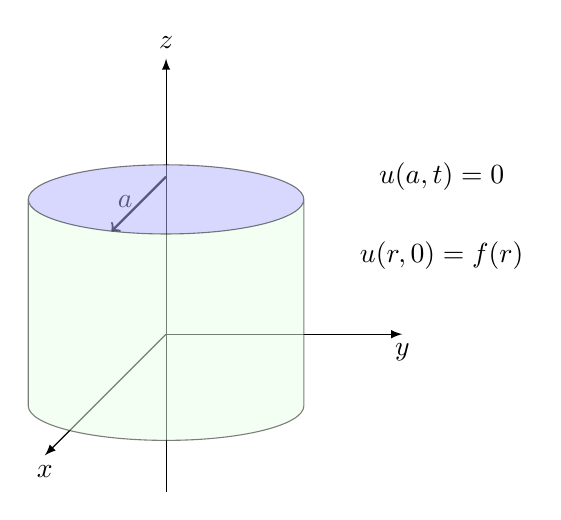
\begin{tikzpicture}
    \coordinate (O) at (0,0,0);
    \coordinate (A) at (3,0,0);
    \coordinate (B) at (0,3.5,0);
    \coordinate (C) at (0,0,4);
    \draw (0, 0, 0) -- (0, -2, 0);
    \draw [->, thick, color=black] (0, 2, 0) -- (0, 2, 1.8) node [above, pos=0.75] {$a$};
    % draw axis
    \draw[-latex] (O) -- (A) node[below] {$y$};
    \draw[-latex] (O) -- (B) node[above] {$z$};
    \draw[-latex] (O) -- (C) node[below] {$x$};

    \node[-latex] at (3.5, 2, 0) {$u(a, t) = 0$};
    \node[-latex] at (3.5, 1, 0) {$u(r, 0) = f(r)$};

    \node[cylinder, draw, shape aspect=.75, 
        cylinder uses custom fill, cylinder end fill=blue!30, 
        minimum height=1cm, minimum size=0.7cm,
        cylinder body fill=green!10, opacity=0.5, 
    scale=5, rotate=90] (c) at (0, 0) {};
\end{tikzpicture}
\end{document}